\textbf{Segundo parcial}
\begin{itemize}
%% Teoría blalances diferenciales (mod 4)
\item ¿Bajo qué hipótesis puede aplicarse la ecuación de flujo potencial?
\item ¿Cuál es la definición de la función linea de corriente?
\item ¿Los balances diferenciales representan conservación de propiedades en qué tipo de sistemas?
\item ¿Cuál es la diferencia entre los enfoques Euleriano y Lagrangiano?

%% Teoria flujo externo capa límite y turbulencia (mod 5)
\item Definir el concepto de capa límite. Definir la condición de no deslizamiento.
\item Escriba la fórmula de cálculo para el número de Reynolds. Dé una interpretación de dicho cociente y explique brevemente su relación con la turbulencia.
\item En aerodinámica ¿Qué es la fuerza de drag?¿Qué la produce?
\item Definir el concepto de capa límite. Definir la condición de no deslizamiento.

%% Teoría flujos compresibles (mod 6)
\item ¿Qué es el número de Mach? ¿Cómo se clasifican los flujos en función del valor del mismo?
 \item ¿De qué variables depende la velocidad del sonido en un gas ideal? ¿Qué es el número de Mach? ¿Cómo se clasifican los flujos en función del valor del mismo?
\item ¿De qué depende a velocidad de propagación del sonido en un fluido?
A la misma temperatura y presión ¿el sonido se propaga más rápido en líquidos o gases?
\item Describir las posibles evoluciones del flujo en una tobera convergente divergente. ¿Qué variables determinan el flujo que se desarrolla en la tobera?
%%-----------------------------------------------------------------------
%%Ejercicios Balances diferenciales
%Obtener ecuación de flujo Couette y Poiseuille
\item Se pretende analizar el campo de velocidades para el flujo laminar \textbf{desarrollado} entre dos placas planas \textbf{infinitas}, dado en la figura \ref{fig:placas_paralelas}. Considerando el problema \textbf{estacionario}:
\begin{enumerate}
  \item Defina las hipótesis para aplicar la ecuación de Navier-Stokes \ref{eq:NSMom_u_cart}.
  \item Defina las condiciones de contorno de este problema.
  \item Aplique las simplificaiones de simetría pertinentes.
  \item A partir de los tres apartados anteriores, obtenga la ecuación diferencial simplificada para el campo de velocidades. Explique bajo qué condiciones se obtiene flujo Poiseuille y en qué condiciones se obtiene flujo Couette.
  \item Para cada caso, grafique perfiles de velocidad y de esfuerzo de corte.
\end{enumerate}
\begin{equation}\label{eq:NSMom_u_cart}
\begin{aligned}
\frac{\partial u}{\partial x} + \frac{\partial v}{\partial y} + \frac{\partial w}{\partial z}&= 0
\\
\frac{\partial u}{\partial t} + u\frac{\partial u}{\partial x} + v\frac{\partial u}{\partial y} + w \frac{\partial u}{\partial z} = -\frac{1}{\rho}\frac{\partial p}{\partial x} + \nu \left(\frac{\partial^2 u}{\partial x^2} + \frac{\partial^2 u}{\partial y^2} + \frac{\partial^2 u}{\partial z^2}\right)
\end{aligned}
\end{equation}

\begin{figure}[h!!]
\centering
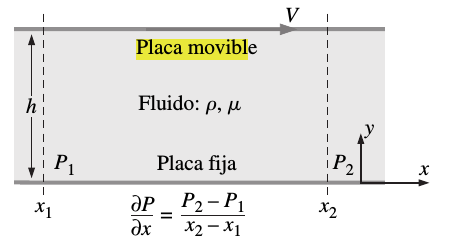
\includegraphics[width=0.6\textwidth]{placas_paralelas.png}
\caption{Flujo entre placas paralelas}
\label{fig:placas_paralelas}
\end{figure}

%% Flujo Hagen Poiseuille
\item Se pretende analizar el campo de velocidades para el flujo laminar \textbf{desarrollado} en una cañería cilíndrica \textbf{infinita}, dado en la figura \ref{fig:hagen_poiseuille}. Considerando el problema \textbf{estacionario}:
\begin{enumerate}
  \item Defina las hipótesis para aplicar la ecuación de Navier-Stokes \ref{eq:NSMom_u_cil}.
  \item Defina las condiciones de contorno de este problema.
  \item Aplique las simplificaiones de simetría pertinentes.
  \item A partir de los tres apartados anteriores, obtenga la ecuación diferencial simplificada para el campo de velocidades.
  \item A partir de la solución, exprese el caudal flujado en función de los datos del problema.
\end{enumerate}

\begin{equation}\label{eq:NSMom_u_cil}
\begin{aligned}
\frac{1}{r}\frac{\partial }{\partial r} (r\,u_r)+ \frac{1}{r}\frac{\partial u_\theta}{\partial \theta} + \frac{\partial u_z}{\partial z}
&= 0 
\\
\frac{\partial u_z}{\partial t} + u_r\frac{\partial u_z}{\partial r} + \frac{u_\theta}{r}\frac{\partial u_z}{\partial \theta} + u_z \frac{\partial u_z}{\partial z} = -\frac{1}{\rho}\frac{\partial p}{\partial z}
%+ \nu \left(\frac{1}{r}\frac{\partial}{\partial r}\left(r\frac{\partial u_z}{\partial r}\right) + \left(\frac{1}{r^2}\frac{\partial^2 u_z}{\partial \theta^2} + \frac{\partial^2 u}{\partial z^2}\right)
\end{aligned}
\end{equation}

\begin{figure}[h!!]
\centering
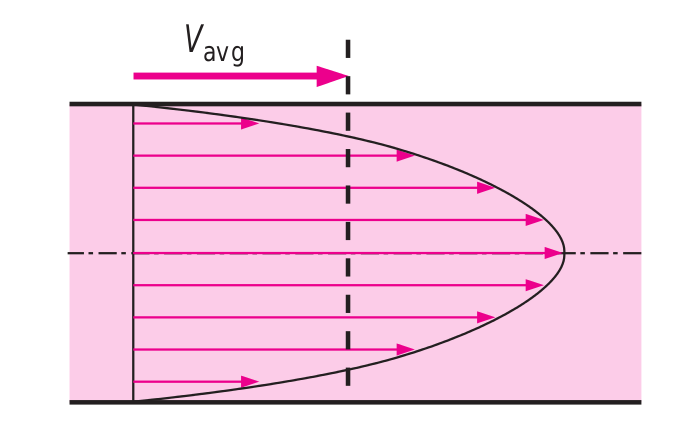
\includegraphics[width=0.6\textwidth]{hagen_poiseuille.png}
\caption{Flujo en un conducto cilíndrico}
\label{fig:hagen_poiseuille}
\end{figure}

%% Drag sobre placa plana
\item El auto de la figura \ref{fig:auto_placa} transporta una placa de madera de dimenesiones ($L = 4$m X $b =3$m) y espesor despreciable, moviéndose a una velocidad de 100 km/h. Calcule el espesor de capa límite en el extremo final de la tabla y la fuerza total de drag para régimen laminar y turbulento. ¿Cuál de los dos resultados es más preciso?
\begin{figure}[h!!]
\centering
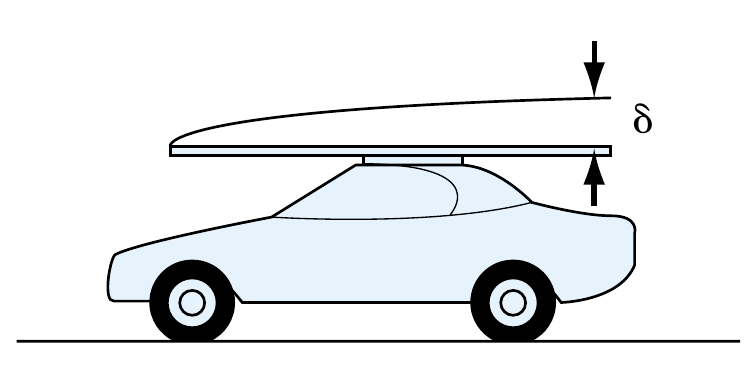
\includegraphics[width=0.4\textwidth]{auto_placa.png}
\caption{Auto transportando la placa de madera de $L$ X $b$}
\label{fig:auto_placa}
\end{figure}


%% Pitot en capa límite
\item La figura \ref{fig:capa_limite} muestra la ubicación de un tubo de pitot en una superficie plana que se desplaza a una velocidad $U = 5$ km/h. Utilizando la solución de capa límite de Blasius, calcular la diferencia de presión que medirá el Pitot. Recuerde que la misma corresponde a la presión dinámica del flujo $p_{din} = \rho u^2/2$. A la distancia $L$, ¿cuál es el espesor de capa límite?

Una solución aproximada a la ecuación de Blasius es el polinomio de cuarto orden dado por la ecuación \ref{eq:PolBlasius}. A continuación se listan los datos del flujo:
\begin{center}
$\rho = 1.2 kg/m^3 \qquad \mu =1.75 \times 10^{-05} Pa s\qquad L = 0.1 m \qquad h = 0.001 m$
\end{center}

\begin{equation}\label{eq:PolBlasius}
u/U = 0.0016217 \eta^4 - 0.0190921 \eta^3 + 0.0314731 \eta^2 + 0.3146989 \eta + 0.0015430 \qquad \qquad \eta = y \sqrt{\frac{U}{x\nu}}
%%  -9.2735e-05   1.5884e-03  -8.5280e-03   1.0741e-02  -8.2920e-03   3.3435e-01  -7.2436e-05 %% Mayor orden: 6
\end{equation}

\begin{figure}[h!!]
\centering
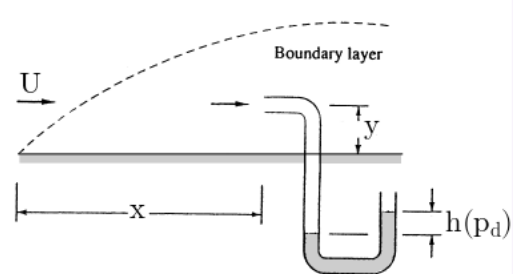
\includegraphics[width=0.4\textwidth]{capa_limite.png}
\caption{Pitot en placa plana, midiendo a una altura $h$}
\label{fig:capa_limite}
\end{figure}

%%Tobera convergente-divergente, sacado del Cimbala:
\item Entra aire a una tobera convergente-divergente, como se muestra en la figura \ref{fig:toberaConvDiv}, a $p_0$ y $T_0$ con velocidad despreciable. El flujo es estacionario, unidimensional e isentrópico con $k = 1.4$. Para obtener un Mach de salida $p_e$, dada una garganta de área $A*$, determinar:
\begin{enumerate}
\item Las condiciones de flujo en la garganta
\item Las condiciones del flujo en el plano de la salida, inclusive el área de la salida de diseño ($Ma_e$, $v_e$, $T_e$).
\item El flujo másico que circula por la tobera.
\item En qué regiones el flujo es sónico y en cuáles supersónico.
\end{enumerate}
\begin{figure}[h!!]
\centering
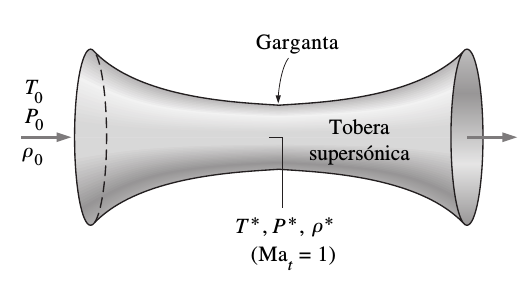
\includegraphics[width=0.5\textwidth]{toberaConvDiv.png}
%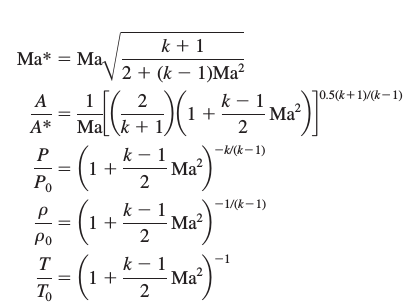
\includegraphics[width=0.5\textwidth]{eqs_comp.png}
\caption{Tobera convergente divergente}
\label{fig:toberaConvDiv}
\end{figure}
\begin{equation*}
\begin{aligned}
\frac{A}{A^*} = \frac{1}{\text{Ma}}\left[\left(\frac{2}{k+1}\right) \left(1 + \frac{k-1}{2}\text{Ma}^2\right)\right]^{0.5(k+1)/(k-1)}
\qquad
\frac{T}{T_0} = \left(1 + \frac{k-1}{2}\text{Ma}^2\right)^{-1}
\\
\frac{p}{p_0} = \left(1 + \frac{k-1}{2}\text{Ma}^2\right)^{-k/(k-1)}
\qquad
\frac{\rho}{\rho_0} = \left(1 + \frac{k-1}{2}\text{Ma}^2 \right)^{-1/(k-1)}
\end{aligned}
\end{equation*}


\end{itemize}
